\subsection{Latency}
\label{sec:hash-timing}
\note{We might need to delete this section since the overlapped parts are too small, we can't make an argument about latency}

We use the same relative latency definition to calculate the latency distribution of MD5s in each feed, and the calculation is based on the shared data between feeds. Since MD5s are not transient, we don't need to set a time restriction for this computation. Figure~\ref{fig:md5-latency} shows the latency distribution CDF of the feeds.

\begin{figure}[h]
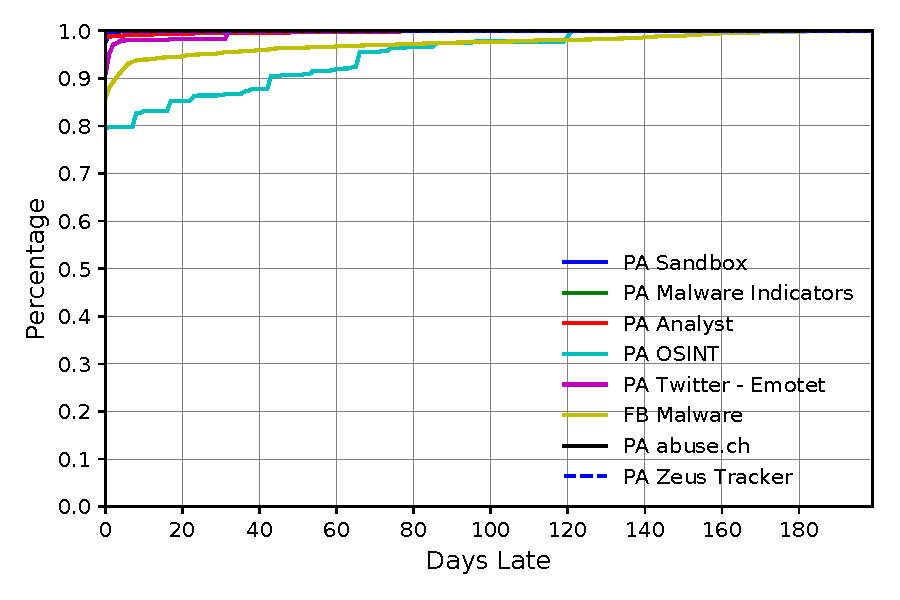
\includegraphics[width=0.9\columnwidth]{images/md5_lateDay.pdf}
\caption{Feed Latency Distribution showing what percentage of each feed's intersected samples are on a particular delay.}
\label{fig:md5-latency}
\end{figure}

As seen in Figure~\ref{fig:md5-latency}, the feeds are roughly grouped into 3 areas. {PA Malware Indicators}, {PA Zeus Tracker}, {PA Analyst}, {PA Twitter - Emotet}, {PA abuse.ch} and {PA Sandbox} report over 90\% of their data first, while {FB Malware }reports over 85\% of its data first. PA OSINT is the outlier in the graph which reports only 80\% of its shared data first. It also has the largest delays, taking almost 50 days to reach 90th percentile and over 70 days to reach 95th percentile.

\finding\ The latency analysis shows which feed is more effective from a timing standpoint, and again demonstrates the fact that a large \ti\ source is not always the quickest at reporting threats.
